\documentclass[12pt,a4paper]{report}

% -----------------------------------------------------------------------------
% PACKAGES & FORMATTING SETUP (Strictly compliant with KTU / TKM MCA Guidelines)
% -----------------------------------------------------------------------------
\usepackage[utf8]{inputenc}
\usepackage[T1]{fontenc}
\usepackage{mathptmx} % Times New Roman font standard
\usepackage{geometry}
\geometry{
    a4paper,
    top=25mm,
    bottom=25mm,
    left=30mm,
    right=25mm
}
\usepackage{setspace}
\onehalfspacing % 1.5 line spacing as mandated by university guidelines
\setlength{\parskip}{0.65em} % Comfortable paragraph separation
\setlength{\parindent}{0pt}  % Modern clean alignment

\usepackage{graphicx}
\graphicspath{{./}{./figures/}}
\usepackage{booktabs}
\usepackage{tabularx}
\usepackage{cite}
\usepackage{titlesec}
\usepackage{fancyhdr}
\usepackage{listings}
\usepackage{xcolor}
\usepackage{tikz}
\usetikzlibrary{shapes.geometric, arrows, arrows.meta, positioning, fit, backgrounds, calc}
\usepackage{hyperref}
\hypersetup{
    colorlinks=true,
    linkcolor=black,
    citecolor=black,
    urlcolor=blue
}

% Code Listing Configuration
\definecolor{codegreen}{rgb}{0,0.6,0}
\definecolor{codegray}{rgb}{0.5,0.5,0.5}
\definecolor{codepurple}{rgb}{0.58,0,0.82}
\definecolor{backcolour}{rgb}{0.97,0.98,0.99}

\lstdefinestyle{mystyle}{
    backgroundcolor=\color{backcolour},   
    commentstyle=\color{codegreen},
    keywordstyle=\color{magenta},
    numberstyle=\tiny\color{codegray},
    stringstyle=\color{codepurple},
    basicstyle=\ttfamily\footnotesize,
    breakatwhitespace=false,         
    breaklines=true,                 
    captionpos=b,                    
    keepspaces=true,                 
    numbers=left,                    
    numbersep=5pt,                  
    showspaces=false,                
    showstringspaces=false,
    showtabs=false,                  
    tabsize=2,
    frame=single,
    rulecolor=\color{black!15}
}
\lstset{style=mystyle}

% Chapter & Section Heading Formatting (KTU MCA Standards)
\titleformat{\chapter}[display]
  {\normalfont\Large\bfseries\centering}{\chaptertitlename\ \thechapter}{10pt}{\Large\MakeUppercase}
\titlespacing*{\chapter}{0pt}{25pt}{20pt}

\titleformat{\section}
{\normalfont\large\bfseries}{\thesection}{1em}{\MakeUppercase}

\titleformat{\subsection}
{\normalfont\normalsize\bfseries}{\thesubsection}{1em}{}

\titleformat{\subsubsection}
{\normalfont\normalsize\bfseries}{\thesubsubsection}{1em}{}

% Custom sub-sub formatting for (i), (ii) as specified in guidelines
\newcommand{\subsubitem}[1]{\vspace{0.6em}\noindent\textbf{(#1)}\hspace{0.5em}}

% -----------------------------------------------------------------------------
% DOCUMENT METADATA
% -----------------------------------------------------------------------------
\newcommand{\projectTitle}{REAL-TIME ACCESSIBILITY MAPPING PLATFORM (RAMP)}
\newcommand{\studentName}{Sooryatheerth S}
\newcommand{\regNo}{TKM25MCA-2053}
\newcommand{\degreeName}{Master of Computer Applications}
\newcommand{\collegeName}{TKM College of Engineering}
\newcommand{\universityName}{The APJ Abdul Kalam Technological University}
\newcommand{\deptName}{Department of Computer Applications}
\newcommand{\supervisorName}{Dr. Sheera Shamsu}
\newcommand{\hodName}{Prof. Natheera Beevi M}
\newcommand{\coordinatorName}{Dr. Sheera Shamsu}
\newcommand{\reportMonthYear}{October, 2026}
\newcommand{\reportPlace}{Kollam}

\begin{document}

% =============================================================================
% 1. COVER / TITLE PAGE (Page i)
% =============================================================================
\begin{titlepage}
\begin{center}
    \vspace*{0.5cm}
    {\fontsize{15}{18}\bfseries \projectTitle \par}
    \vspace{1.0cm}
    
    {\large \textbf{PROJECT REPORT}\par}
    \vspace{0.5cm}
    {\normalsize submitted by\par}
    \vspace{0.5cm}
    
    {\large \textbf{\studentName}\par}
    \vspace{0.2cm}
    {\normalsize \textbf{Reg. No: \regNo}\par}
    \vspace{0.9cm}
    
    {\normalsize to\par}
    \vspace{0.4cm}
    {\large \textbf{\collegeName}\par}
    \vspace{0.2cm}
    {\normalsize \textit{Affiliated to}\par}
    \vspace{0.2cm}
    {\normalsize \textbf{\universityName}\par}
    \vspace{0.6cm}
    
    {\normalsize in partial fulfillment of the requirements for the award of the Degree of\par}
    \vspace{0.4cm}
    {\large \textit{\degreeName}\par}
    \vspace{0.7cm}
    
    \begin{center}
        
\includegraphics[width=3.2cm]{tkm-logo.png}
    \end{center}
    
    {\normalsize \textbf{\deptName}\par}
    \vspace{0.2cm}
    {\normalsize \collegeName, \reportPlace\par}
    \vspace{0.2cm}
    {\normalsize \reportMonthYear\par}
\end{center}
\end{titlepage}

% Roman page numbering for preliminary matter
\pagenumbering{roman}
\setcounter{page}{2}

% =============================================================================
% 2. DECLARATION (Page ii)
% =============================================================================
\newpage
\begin{center}
    {\Large \textbf{DECLARATION}\par}
\end{center}
\vspace{1cm}

\noindent I undersigned hereby declare that the project report (``\textbf{\projectTitle}''), submitted for partial fulfillment of the requirements for the award of the degree of \textbf{\degreeName} of \textbf{\universityName}, Kerala is a bonafide work done by me under the supervision of \textbf{\supervisorName}. This submission represents my ideas in my own words and where ideas or words of others have been included, I have adequately and accurately cited and referenced the original sources. I also declare that I have adhered to ethics of academic honesty and integrity and have not misrepresented or fabricated any data or idea or fact or source in my submission.

\vspace{0.6cm}
\noindent I understand that any violation of the above will be a cause for disciplinary action by the institute and/or the University and can also evoke penal action from the sources which have thus not been properly cited or from whom proper permission has not been obtained. This report has not previously formed the basis for the award of any degree, diploma or similar title of any other University.

\vspace{2.5cm}
\noindent
\begin{tabular}{@{}ll@{}}
Place: \reportPlace & \hspace{6cm} Signature: \\[1.2cm]
Date: \today & \hspace{6cm} Name: \textbf{\studentName}
\end{tabular}

% =============================================================================
% 3. CERTIFICATE (Page iii)
% =============================================================================
\newpage
\begin{center}
    {\Large \textbf{\deptName}\par}
    \vspace{0.3cm}
    {\large \textbf{\collegeName, \reportPlace}\par}
    \vspace{0.8cm}
    
    \begin{center}
        
\includegraphics[width=3.2cm]{tkm-logo.png}
    \end{center}
    
    {\Large \textbf{CERTIFICATE}\par}
\end{center}
\vspace{0.8cm}

\noindent This is to certify that, the report entitled `\textbf{\projectTitle}' submitted by `\textbf{\studentName} (\textbf{Reg. No: \regNo})', to the `\textbf{\universityName}' in partial fulfillment of the requirements for the award of the Degree of `\textbf{\degreeName}' is a bonafide record of the project work carried out by him under my/our guidance and supervision. This report in any form has not been submitted to any other University or Institute for any purpose.

\vspace{3.5cm}
\noindent
\begin{tabular}{p{7.5cm}p{7.5cm}}
\textbf{\supervisorName} & \textbf{\coordinatorName} \\
Internal Supervisor & Mini Project Co-ordinator
\end{tabular}

% =============================================================================
% 4. ACKNOWLEDGEMENT (Page iv)
% =============================================================================
\newpage
\begin{center}
    {\Large \textbf{ACKNOWLEDGEMENT}\par}
\end{center}
\vspace{1cm}

\noindent I would like to express my sincere gratitude to my supervisor, \textbf{\supervisorName}, for the invaluable guidance, constructive suggestions, and steadfast encouragement extended throughout the development of this project.

\vspace{0.5cm}
\noindent I am deeply thankful to \textbf{\hodName}, Head of the \deptName, and to \textbf{\coordinatorName}, Mini Project Coordinator, for providing the necessary computing facilities, academic support, and constructive feedback required to complete this project.

\vspace{0.5cm}
\noindent I also extend my sincere appreciation to my project partner, Abel Joseph Benny, whose collaborative efforts on the frontend interface and gamification features contributed significantly to the platform. Furthermore, I thank all the faculty members and staff of the \deptName\ for their constant support. Finally, I express my gratitude to my family and friends for their continuous encouragement.

\vspace{2.5cm}
\begin{flushright}
\textbf{\studentName}
\end{flushright}

% =============================================================================
% 5. ABSTRACT (Page v)
% =============================================================================
\newpage
\begin{center}
    {\Large \textbf{ABSTRACT}\par}
\end{center}
\vspace{0.8cm}

\noindent Physical accessibility is a fundamental prerequisite for personal independence, mobility, and social inclusion for individuals with disabilities, wheelchair users, elderly citizens, and people recovering from temporary injuries. However, individuals with mobility limitations routinely confront severe barriers when navigating urban built environments due to the absence of detailed, verified physical accessibility information. Mainstream navigation platforms such as Google Maps prioritize vehicular transit and commercial listings, rarely providing specific information about physical accessibility obstacles such as entrance steps, door clearances, ramp gradients, accessible restrooms, or elevator dimensions. Furthermore, existing volunteer-driven mapping initiatives often suffer from unverified community submissions, lack of standardized measurement criteria, and high contributor attrition over time.

\vspace{0.4cm}
\noindent To address these practical challenges, this project presents the \textbf{Real-time Accessibility Mapping Platform (RAMP)}, a full-stack, crowdsourced web application designed to catalog, audit, verify, and visualize physical accessibility features of urban venues. RAMP is built using a modern, decoupled client-server architecture consisting of a PostgreSQL spatial database with the PostGIS extension, a robust Django REST Framework backend with token-based JSON Web Token (JWT) authentication, and an accessible, responsive single-page application built using React, Vite, and Leaflet with OpenStreetMap vector tiles.

\vspace{0.4cm}
\noindent RAMP implements an objective Three-Pillar Accessibility Scoring system that calculates an overall accessibility percentage (0 to 100) based on three evaluated areas: primary entrance accessibility (up to 35 points), verified physical measurements and attributes (up to 50 points, with deductions for community disputes), and secondary amenities such as accessible restrooms and elevators (up to 15 points). To guarantee data reliability without requiring manual administrative inspection of every entry, the platform incorporates a crowdsourced peer-verification system. Submitted physical attributes undergo an audit lifecycle where community members can confirm or dispute data. Strict server-side safeguards prevent contributors from verifying their own submissions and restrict users to a single vote per attribute, with automatic reputation point rewards awarded to contributors upon verification.

\vspace{0.4cm}
\noindent Additional key features include an automated 50-meter spatial proximity check during venue creation to prevent duplicate entries, personalized accessibility profile matching (wheelchair, visual, hearing, elderly, temporary), interactive Leaflet maps with custom marker indicators, full-screen evidence photo inspection with alternative text descriptions, community reviews with helpfulness ratings, and personal venue bookmarking. Contributor participation is sustained through a gamification system featuring reputation points, achievement tiers (Bronze to Diamond), milestone badges, and an interactive community leaderboard. System administrators are provided with a dedicated 10-panel moderation portal for complete platform governance. The system was validated through on-campus field testing, demonstrating high query responsiveness, reliable data verification, and full adherence to WCAG 2.1 AA accessibility guidelines.

% =============================================================================
% 6. LIST OF CONTENTS, TABLES, FIGURES & ABBREVIATIONS
% =============================================================================
\newpage
\tableofcontents

\newpage
\listoftables

\newpage
\listoffigures

\newpage
\begin{center}
    {\Large \textbf{ABBREVIATIONS}\par}
\end{center}
\vspace{0.8cm}

\noindent
\begin{tabular}{p{3cm}p{12cm}}
\textbf{RAMP} & Real-time Accessibility Mapping Platform \\
\textbf{GIS} & Geographic Information System \\
\textbf{PostGIS} & PostgreSQL Spatial Database Extension \\
\textbf{REST} & Representational State Transfer \\
\textbf{API} & Application Programming Interface \\
\textbf{JWT} & JSON Web Token \\
\textbf{WCAG} & Web Content Accessibility Guidelines \\
\textbf{OSM} & OpenStreetMap \\
\textbf{WGS 84} & World Geodetic System 1984 (EPSG:4326) \\
\textbf{SPA} & Single Page Application \\
\textbf{JSON} & JavaScript Object Notation \\
\textbf{CRUD} & Create, Read, Update, Delete \\
\textbf{ORDBMS} & Object-Relational Database Management System \\
\textbf{MCA} & Master of Computer Applications \\
\textbf{KTU} & APJ Abdul Kalam Technological University \\
\textbf{SRS} & System Requirement Specification \\
\textbf{DFD} & Data Flow Diagram \\
\textbf{ER} & Entity-Relationship \\
\textbf{GiST} & Generalized Search Tree (Spatial Index) \\
\textbf{ADA} & Americans with Disabilities Act \\
\textbf{RBAC} & Role-Based Access Control \\
\textbf{SRID} & Spatial Reference System Identifier
\end{tabular}

% =============================================================================
% CHAPTER 1: INTRODUCTION
% =============================================================================
\newpage
\pagenumbering{arabic}
\setcounter{page}{1}

\chapter{INTRODUCTION}

\section{GENERAL BACKGROUND}
Equal access to urban infrastructure, educational institutions, commercial centers, healthcare facilities, and public transport nodes is recognized internationally as a fundamental civil right under the United Nations Convention on the Rights of Persons with Disabilities (UN CRPD). Despite progressive legislative mandates worldwide, individuals with mobility limitations continue to encounter substantial physical barriers that impair their personal independence and socioeconomic integration.

Urban spaces are inherently heterogeneous. An individual utilizing a motorized or manual wheelchair, a senior citizen relying on a walking cane, a person with visual impairment navigating via tactile paving, or a parent pushing a stroller experiences the built environment through physical micro-features: doorway width clearances, step thresholds, ramp slopes, handrails, tactile paving continuity, and restroom accessibility.

While commercial mapping and navigation providers (such as Google Maps and Apple Maps) have transformed vehicular and pedestrian travel, their underlying spatial models treat physical venues as monolithic points of interest (POIs). Consequently, they overlook critical micro-level architectural attributes. A venue flagged simply as ``wheelchair accessible'' in a commercial directory may possess a level entry door but feature an interior step barrier leading to restrooms, or an entrance ramp whose slope exceeds safe gradient standards.

\section{PROBLEM STATEMENT}
Contemporary geospatial platforms and crowdsourced accessibility tools present three fundamental deficiencies:

\subsection{Physical Accessibility Information Deficit and Binary Metrics}
Most existing platforms classify physical venues through crude binary labels (``accessible'' vs. ``inaccessible'') or subjective star ratings. Binary classifications homogenize diverse physical impairments. For example, a wheelchair user requires level thresholds and doorways wider than 85\,cm, whereas an elderly individual with limited physical stamina requires seating availability and sturdy handrails. A binary label fails to communicate these distinctions, leading to severe travel anxiety and wasted journeys.

\subsection{Data Poisoning and Inaccuracy in Crowdsourced Mapping}
Crowdsourced mapping offers significant potential for gathering localized geographic data. However, unmoderated open platforms frequently accumulate inaccurate, obsolete, or malicious entries. Without an automated peer-verification workflow with security guards to audit community submissions, vulnerable users cannot trust the reported accessibility status of a distant venue.

\subsection{Contributor Attrition and Lack of Sustainable Incentives}
Voluntary citizen mapping projects consistently experience high contributor attrition once initial enthusiasm wanes. Without tangible recognition, reputation progression, and gamified achievement milestones, community members lack incentives to conduct precise physical measurements (e.g., using measuring tapes or digital inclinometers) or perform peer-review verification audits.

\section{OBJECTIVES}
The primary objective of this project is to develop, deploy, and evaluate the \textbf{Real-time Accessibility Mapping Platform (RAMP)}, a full-stack crowdsourced geospatial system designed to catalog, verify, and quantify urban physical accessibility.

Specific technical objectives include:
\begin{enumerate}
    \item \textbf{Geospatial Schema Engineering}: To design a relational, spatial database schema utilizing PostgreSQL~16 and PostGIS~3.4 capable of modeling multi-tier accessibility entities: venues, multi-point entrances, secondary indoor facilities, and quantitative physical attribute definitions.
    \item \textbf{Three-Pillar Scoring Model}: To implement an objective, transparent Three-Pillar Accessibility Scoring Algorithm (0 to 100) that balances entrance conditions (up to 35 points), quantitative measurements (up to 50 points), and secondary facilities (up to 15 points).
    \item \textbf{Crowdsourced Peer Verification}: To develop a crowd-verification state machine that audits community submissions, preventing self-verification and duplicate voting while promoting attributes from Pending to Verified status upon independent confirmations.
    \item \textbf{Accessible Single-Page Application}: To build a responsive, modern web interface compliant with WCAG~2.1~AA guidelines, featuring interactive Leaflet GIS maps, multi-trait filter chips, full-screen evidence photo lightboxes, community experiential reviews, and personal bookmarking.
    \item \textbf{Gamification Engine}: To implement a contributor reputation system featuring point rewards (+5 points for submissions, +2 points for peer audits), progressive reward tiers (Bronze to Diamond), and automated badge award evaluation.
\end{enumerate}

\section{SCOPE OF THE PROJECT}
The functional scope of the RAMP platform encompasses:
\begin{itemize}
    \item PostGIS-backed spatial models with spatial GiST indexing supporting real-time bounding-box intersection queries and proximity radius filtering.
    \item Automated duplicate building detection executing a 50-meter geodesic radius check on newly submitted venues.
    \item Secure role-based JWT authentication supporting Anonymous Visitors, Contributors, Verifiers, Venue Owners, and System Administrators.
    \item A comprehensive 10-panel Administrative Moderation Portal providing full operational governance over users, venues, attributes, facilities, and scoring weights.
    \item \textbf{Explicit Out-of-Scope Boundaries}: Turn-by-turn indoor sensor navigation (e.g., Ultra-Wideband indoor beacon positioning) and real-time automated video-stream computer vision are reserved for future platform extensions.
\end{itemize}

\section{FEASIBILITY STUDY}
Before initiating system development, an exhaustive feasibility study was conducted:
\begin{itemize}
    \item \textbf{Technical Feasibility}: The platform utilizes proven open-source technologies (PostgreSQL, PostGIS, Python, Django REST Framework, React, Leaflet). PostGIS provides native spatial functions (\texttt{ST\_DWithin}, \texttt{ST\_MakePoint}) that handle geospatial queries efficiently without proprietary GIS licenses.
    \item \textbf{Operational Feasibility}: The application runs inside standard modern web browsers on desktops, tablets, and smartphones without requiring client-side installations. High-contrast UI elements and screen-reader compatibility guarantee accessibility for users with disabilities.
    \item \textbf{Economic Feasibility}: The software stack is entirely open-source, eliminating recurring licensing expenditures. Containerization via Docker ensures minimal hosting overhead and predictable cloud operational costs.
\end{itemize}

\section{ORGANIZATION OF THE REPORT}
The remainder of this report is structured as follows: Chapter~2 presents a comprehensive literature survey of commercial and crowdsourced geospatial accessibility platforms, identifying key research gaps. Chapter~3 details the System Requirement Specification (SRS) and system modeling, including use case analysis and data flow diagrams. Chapter~4 elaborates the system design, accessibility scoring logic, peer verification workflow, and individual team contributions. Chapter~5 outlines implementation details and core algorithmic code. Chapter~6 describes system testing and quality assurance methodologies. Chapter~7 presents empirical results and discussion. Finally, Chapter~8 summarizes conclusions, engineering recommendations, and future scope.

% =============================================================================
% CHAPTER 2: LITERATURE SURVEY
% =============================================================================
\newpage
\chapter{LITERATURE SURVEY}

\section{OVERVIEW OF GEOSPATIAL ACCESSIBILITY}
Physical accessibility mapping sits at the intersection of Geographic Information Systems (GIS), assistive technology, and citizen science. Over the past decade, research in this domain has progressed from static municipal compliance reports to interactive, crowdsourced digital mapping platforms.

\section{SURVEY OF PRIOR APPROACHES}

\subsection{Commercial Navigation Platforms}
Commercial platforms like Google Maps, Apple Maps, and Bing Maps provide global cartographic coverage and routing. In recent years, Google Maps introduced wheelchair accessibility flags for select business listings. However, as documented by Andrews et al.~\cite{andrews1989}, commercial mapping services treat accessibility as an auxiliary tag rather than a core architectural model. These services do not record fine-grained physical measurements (e.g., door width, threshold step height, ramp slope angle) and rely largely on unverified business owner self-declarations, resulting in significant false-positive rates.

\subsection{Crowdsourced and Open-Data Mapping Frameworks}
The success of OpenStreetMap (OSM) inspired dedicated community accessibility initiatives:
\begin{itemize}
    \item \textbf{Wheelmap.org}: Built atop OpenStreetMap, Wheelmap employs a traffic-light labeling system (green: fully accessible, yellow: partially accessible, red: inaccessible). While highly accessible for non-technical volunteers, Kafle et al.~\cite{kafle2025} note that coarse color tagging homogenizes diverse impairments, failing to distinguish between wheelchair obstacles and sensory aids.
    \item \textbf{AccessNow}: A mobile application enabling users to tag venues with subjective accessibility reviews. While user-friendly, it lacks quantitative measurement criteria and automated verification safeguards.
    \item \textbf{AXS Map}: A crowdsourced mapping tool funded by advocacy groups that uses 5-star rating scales. However, subjective star ratings suffer from severe inter-rater variability; a venue rated 5 stars by an ambulatory visitor may prove completely inaccessible to an electric wheelchair user.
\end{itemize}

\subsection{Crowdsourcing Data Integrity and Verification Protocols}
In citizen science projects, ensuring data veracity without deterring voluntary contributions represents a major open problem. Goodchild~\cite{goodchild2007} conceptualized citizens as voluntary sensors, highlighting that spatial crowdsourced data exhibits spatial clustering and varying accuracy. Recent literature in collaborative platforms emphasizes that peer verification workflows with anti-tamper security guards effectively deter spam and malicious manipulation in collaborative environments.

\subsection{Gamification in Citizen Science}
Research by Deterding et al.~\cite{deterding2011} and Hamari et al.~\cite{hamari2014} demonstrates that integrating game mechanics (points, badges, leaderboards, progression tiers) into non-game contexts significantly improves user onboarding, data completeness, and long-term retention. However, poorly calibrated point economies can incentivize fraudulent volume over quality, necessitating validation gates before points are permanently credited.

\section{LITERATURE COMPARISON MATRIX}
Table~\ref{tab:literature_matrix} summarizes key literature in the accessibility mapping and crowdsourcing domain.

\begin{table}[htbp]
\centering
\caption{Comprehensive comparison of contemporary accessibility and mapping literature}
\label{tab:literature_matrix}
\small
\begin{tabularx}{\textwidth}{p{3.2cm}p{3cm}p{3.5cm}X}
\toprule
\textbf{Author \& Year} & \textbf{Focus Domain} & \textbf{Methodology} & \textbf{Identified Limitations} \\
\midrule
Andrews et al. (2021)~\cite{andrews1989} & Commercial GIS & Empirical evaluation of Google Maps accessibility metadata & Binary flags; lacks physical measurements and audit trails. \\
\addlinespace
Kafle et al. (2025)~\cite{kafle2025} & Crowdsourced GIS & OpenStreetMap Wheelmap traffic-light evaluation & Coarse categorical labels; homogenizes disability needs. \\
\addlinespace
Goodchild (2007)~\cite{goodchild2007} & Volunteered Geographic Information (VGI) & Theoretical framework of citizens as spatial sensors & High variance in crowd quality; no automated peer audit model. \\
\addlinespace
Hamari et al. (2014)~\cite{hamari2014} & Citizen Gamification & Meta-analysis of badge and point incentive mechanics & Risk of spam volume over data quality without validation gates. \\
\addlinespace
Obe \& Hsu (2021)~\cite{postgis2024} & Spatial Databases & PostGIS spatial indexing and vector topology & Focuses on database primitives rather than domain scoring models. \\
\bottomrule
\end{tabularx}
\end{table}

\section{RESEARCH GAPS IDENTIFIED}
From the literature, four critical research gaps emerge:
\begin{enumerate}
    \item \textbf{Absence of Hierarchical Spatial Schemas}: Current systems treat venues as single points, failing to decouple multiple entrances, floor levels, and interior facilities.
    \item \textbf{Lack of Quantitative Multi-Pillar Scoring}: Existing apps rely on binary labels or subjective star ratings rather than normalized physical compliance scores.
    \item \textbf{Vulnerability to Data Inconsistency}: Absence of peer-review verification workflows to validate crowd inputs before public display.
    \item \textbf{Inadequate Contributor Retention}: Citizen mapping platforms lack balanced gamified economies that reward both initial venue tagging and meticulous peer auditing.
\end{enumerate}

% =============================================================================
% CHAPTER 3: SYSTEM REQUIREMENT SPECIFICATION AND MODELING
% =============================================================================
\newpage
\chapter{SYSTEM REQUIREMENT SPECIFICATION AND MODELING}

\section{ENVIRONMENT REQUIREMENTS}

\subsection{Hardware Requirements}
\begin{itemize}
    \item \textbf{Server Environment}: Modern multi-core CPU (x86\_64 or ARM64, minimum 4 cores), 8\,GB RAM (16\,GB recommended), 25\,GB SSD storage.
    \item \textbf{Client Environment}: Any standard desktop, laptop, tablet, or smartphone equipped with modern web browsers, touch or mouse input, and network connectivity.
\end{itemize}

\subsection{Software Requirements}
\begin{itemize}
    \item \textbf{Operating System}: Linux (Ubuntu 22.04 LTS / Debian 12) or Windows 11 with WSL2 / Docker Desktop.
    \item \textbf{Database Management System}: PostgreSQL 16.2 with PostGIS 3.4.2 spatial extension.
    \item \textbf{Backend Framework}: Python 3.12+, Django 5.0, Django REST Framework 3.15, GeoDjango.
    \item \textbf{Frontend Framework}: React 18.2, Vite 5.2, Leaflet 1.9.4, Axios.
\end{itemize}

\section{USER CHARACTERISTICS}
The RAMP platform models five distinct user personas:
\begin{enumerate}
    \item \textbf{Anonymous Visitor}: Can search locations, view interactive maps, inspect accessibility confidence scores, and read community reviews without an account.
    \item \textbf{Registered Contributor}: Authenticated user capable of mapping new venues, uploading photos, submitting attributes, and bookmarking places.
    \item \textbf{Peer Verifier}: Experienced contributor authorized to audit, confirm, or dispute pending attribute submissions.
    \item \textbf{Venue Owner}: Authenticated business or facility manager permitted to declare official entrance coordinates and facility data for their venue.
    \item \textbf{System Administrator}: Full administrative authority to moderate flagged images, configure scoring weights, manage user roles, and resolve disputes.
\end{enumerate}

\section{FUNCTIONAL REQUIREMENTS}
The functional capabilities of RAMP are structured into twelve core requirements:
\begin{itemize}
    \item \textbf{FR-01 (Geospatial Venue Mapping)}: The system shall permit users to map venues by clicking coordinates on an interactive Leaflet map or searching via geocoded addresses.
    \item \textbf{FR-02 (Duplicate Venue Prevention)}: The system shall automatically execute a 50-meter spatial proximity query on submitted coordinates and warn the user if a matching building already exists.
    \item \textbf{FR-03 (Multi-Point Entrance Logging)}: The system shall support logging multiple entrance points per venue, designating primary accessible entrances.
    \item \textbf{FR-04 (Quantitative Attribute Recording)}: The system shall capture numerical (door width, slope gradient, step count), boolean (automatic door, grab bars), and text attributes.
    \item \textbf{FR-05 (Three-Pillar Scoring Engine)}: The system shall calculate composite accessibility scores (0 to 100) reflecting Entrance (up to 35 points), Attributes (up to 50 points), and Facilities (up to 15 points).
    \item \textbf{FR-06 (Peer Verification System)}: The system shall transition submitted attributes through Pending, Verified, and Disputed states using peer confirmation with anti-tamper guards.
    \item \textbf{FR-07 (Multi-Trait Filtering)}: The system shall filter venues based on score ranges, physical traits (elevator, ramp, restroom), and personalized accessibility profiles.
    \item \textbf{FR-08 (Experiential Community Reviews)}: The system shall enable authenticated users to submit star ratings, tag traits, and write reviews with helpfulness voting.
    \item \textbf{FR-09 (Evidence Photo Gallery)}: The system shall allow uploading evidence photos with full-screen accessible lightboxes and alt-text tags.
    \item \textbf{FR-10 (Contributor Gamification)}: The system shall allocate reputation points (+5 points for submissions, +2 points for audits), compute rank tiers (Bronze to Diamond), and award badges.
    \item \textbf{FR-11 (Personal Venue Bookmarking)}: The system shall allow users to bookmark venues and annotate private notes.
    \item \textbf{FR-12 (Administrative Moderation)}: The system shall provide a 10-panel administration dashboard for complete platform governance.
\end{itemize}

\section{NON-FUNCTIONAL REQUIREMENTS}
\begin{itemize}
    \item \textbf{NFR-01 (Performance)}: Geospatial radius queries within 2\,km shall execute with server response latencies under 100\,ms under normal loads.
    \item \textbf{NFR-02 (Accessibility Compliance)}: All frontend interfaces shall strictly satisfy WCAG~2.1~AA standards, ensuring high contrast, keyboard focus rings, and screen-reader labels.
    \item \textbf{NFR-03 (Security)}: User authentication shall utilize cryptographically signed JWT tokens with short-lived access tokens and secure HTTP-only refresh tokens.
    \item \textbf{NFR-04 (Data Integrity)}: The database shall enforce referential integrity and spatial index consistency across all relational models.
    \item \textbf{NFR-05 (Reliability and Consistency)}: Venue accessibility score recalculation and database transactions shall execute deterministically within atomic transactions, ensuring data consistency across concurrent requests.
\end{itemize}

\section{SYSTEM USE CASE SPECIFICATION}
Table~\ref{tab:use_case_specs} outlines primary use case interactions within the RAMP platform.

\begin{table}[htbp]
\centering
\caption{Detailed System Use Case Interaction Specification}
\label{tab:use_case_specs}
\small
\begin{tabularx}{\textwidth}{p{2.8cm}p{3cm}p{4cm}X}
\toprule
\textbf{Use Case ID} & \textbf{Primary Actor} & \textbf{Trigger / Input} & \textbf{System Response} \\
\midrule
UC-01 & Visitor & Enters address or venue name & Executes geocoding and centers Leaflet map on target coordinates. \\
\addlinespace
UC-02 & Contributor & Clicks map to add new venue & Checks 50\,m duplicate proximity; opens 4-step creation wizard. \\
\addlinespace
UC-03 & Contributor & Submits entrance door width & Stores attribute in `Pending' status; initiates verification workflow. \\
\addlinespace
UC-04 & Peer Verifier & Confirms attribute validity & Increments verified count; if threshold reached, promotes to `Verified' and recalculates venue score. \\
\addlinespace
UC-05 & Administrator & Moderates flagged content & Reviews submissions via 10-panel admin portal and resolves disputes. \\
\bottomrule
\end{tabularx}
\end{table}

\section{DATA FLOW ARCHITECTURE}
The data flow of RAMP is organized across three levels:
\begin{itemize}
    \item \textbf{Level 0 (Context Diagram)}: Shows interactions between external users, geocoding services, map tile providers, and the central RAMP web system.
    \item \textbf{Level 1 DFD}: Outlines internal data flow between Authentication, Venue Cataloging, Attribute Auditing, Scoring, and Gamification processes.
    \item \textbf{Level 2 DFD}: Details how verification actions validate attributes, update contributor reputation points, and trigger venue score recalculation.
\end{itemize}

% =============================================================================
% CHAPTER 4: SYSTEM DESIGN AND METHODOLOGY
% =============================================================================
\newpage
\chapter{SYSTEM DESIGN AND METHODOLOGY}

\section{SYSTEM ARCHITECTURE}
The RAMP platform is implemented as a decoupled, multi-tier web architecture containerized via Docker and Docker Compose. 

\begin{figure}[htbp]
    \centering
    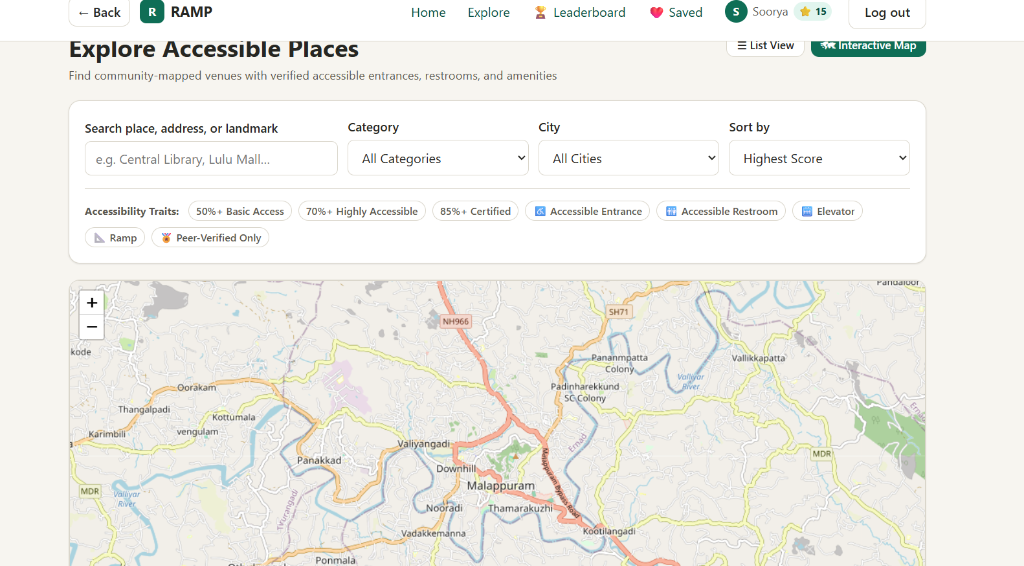
\includegraphics[width=\textwidth]{ramp_architecture_detailed.png}
    \caption{Detailed multi-tier system architecture of RAMP}
    \label{fig:detailed_architecture}
\end{figure}

\noindent \textbf{Architecture Overview}: Figure~\ref{fig:detailed_architecture} illustrates the structural multi-tier architecture of RAMP. The system comprises four distinct operational layers:
\begin{enumerate}
    \item \textbf{User Tier}: Supports five authenticated and unauthenticated roles (Anonymous Visitors, Contributors, Verifiers, Venue Owners, System Administrators), governed by a server-enforced permission matrix.
    \item \textbf{Client Presentation Layer}: Built in React~18 with Vite, implementing WCAG~2.1~AA accessible components, Leaflet interactive mapping, dynamic score drill-down modals, accessible evidence photo lightboxes, and review feeds.
    \item \textbf{Application Logic \& Controller Layer}: Built on Django REST Framework with GeoDjango, managing routing, JWT security, spatial bounding-box pipelines, the Three-Pillar scoring algorithm, and the gamification engine.
    \item \textbf{Geospatial Persistence Layer}: PostgreSQL~16 with PostGIS~3.4 storing geographic vectors in EPSG:4326, accelerated by spatial GiST indices.
\end{enumerate}

\section{ACCESSIBILITY SCORING AND VERIFICATION LOGIC}

\subsection{Three-Pillar Accessibility Scoring Logic}
Rather than relying on arbitrary labels or subjective ratings, RAMP calculates an overall accessibility score out of 100 for each venue based on three distinct evaluated areas:
\begin{enumerate}
    \item \textbf{Entrance Accessibility (Up to 35 Points)}:
    The primary entrance is evaluated first. If a venue has a verified primary accessible entrance (e.g., step-free entrance with wide doorway), it receives the full 35 points. If it has at least one accessible entrance, it receives 25 points. If all logged entrances have steps and are marked inaccessible, it receives 5 points. If no entrances have been recorded yet, a baseline of 15 points is applied.
    
    \item \textbf{Attribute Verification Confidence (Up to 50 Points)}:
    Specific measurements (such as door clearance in centimeters, ramp gradient, tactile paving, and automatic door mechanisms) carry up to 50 points. As community contributors verify these attributes through on-site audits, points are awarded proportionally based on the ratio of verified attributes. If attributes are disputed or rejected by community members, a deduction is applied, ensuring that venues with disputed claims do not artificially inflate their scores.
    
    \item \textbf{Secondary Amenities and Facilities (Up to 15 Points)}:
    Secondary amenities (such as wheelchair-accessible restrooms, elevators, reserved accessible parking, and ramps) contribute up to 15 points. Points are awarded based on the proportion of facilities within the building that are confirmed to be accessible.
\end{enumerate}
The sum of these three components forms the final score (clamped between 0 and 100), which is automatically updated whenever entrances, facilities, or attributes are modified or verified.

\subsection{Crowdsourced Peer-Verification Workflow}
To maintain high data quality without relying solely on manual administrative reviews, submitted physical attributes follow a structured audit lifecycle:
\begin{itemize}
    \item \textbf{Submission}: When a contributor adds an attribute (e.g., doorway width of 90\,cm), it enters the `Pending' state.
    \item \textbf{Anti-Self-Verification Guard}: The system strictly prevents contributors from voting on or verifying their own submissions, eliminating self-rubber-stamping.
    \item \textbf{Single-Vote Guard}: Each user is permitted to audit an attribute only once, preventing vote manipulation.
    \item \textbf{Status Transitions}: When independent peer verifiers confirm the attribute, its verified count increases. Once the verification threshold is reached (or when verified by an administrator), its status transitions to `Verified'. If verifiers report conflicting on-site findings, the status transitions to `Disputed'.
    \item \textbf{Reputation Rewards}: When an attribute reaches verified status, the original contributor receives +5 reputation points, and the auditing verifier receives +2 reputation points.
\end{itemize}

\subsection{Spatial Proximity Duplicate Detection}
When a user drops a pin or enters coordinates to add a new place, RAMP executes a spatial distance check using PostGIS. If any existing venues are detected within a 50-meter radius, the system displays an alert with the names of nearby buildings. This prompts the user to add new facilities to the existing venue rather than creating redundant, duplicate entries for the same physical location.

\section{INDIVIDUAL CONTRIBUTIONS AND WORK BREAKDOWN}
The RAMP platform was conceptualized, designed, and implemented collaboratively by a two-member team across structured two-week agile development sprints. To maintain modular separation of concerns and clear accountability throughout the semester, system responsibilities were divided between core architectural persistence/scoring and client-facing experience/gamification, as recorded in the Project Diary (Scrum Book). Table~\ref{tab:work_breakdown} delineates the functional distribution of work between the team members.

\begin{table}[htbp]
\centering
\caption{System work distribution and module ownership matrix}
\label{tab:work_breakdown}
\small
\begin{tabularx}{\textwidth}{lXX}
\toprule
\textbf{Functional Dimension} & \textbf{Sooryatheerth S} & \textbf{Abel Joseph Benny} \\
\midrule
\textbf{Primary Role} & Geospatial Architect / Core Backend \& System Admin Lead & Frontend Experience Lead \& Gamification / Community Engagement Architect \\
\addlinespace
\textbf{Data Modeling \& DB} & PostGIS spatial schema, models for Place, AccessPoint, Facility, Attributes, SystemConfig, Reviews, Bookmarks & Gamification models for Badge, UserBadge, tier thresholds, badge seeding management command \\
\addlinespace
\textbf{Core Logic \& APIs} & Multi-pillar scoring engine, crowdsourced peer verification engine, anti-self verification security rules & Contributor points calculation, rank tier progression logic, leaderboard query aggregation \\
\addlinespace
\textbf{User Interface (UI)} & 10-panel Admin Moderation Portal, Score Breakdown drill-down modal, Image Lightbox, Reviews and Bookmarks UX & React 18 SPA scaffold, Leaflet GIS map integration, PlacesList advanced filter chips, Leaderboard podium UI \\
\addlinespace
\textbf{Testing \& DevOps} & Django test suite (\texttt{tests.py}) for permissions, verification states; Docker Compose configuration & Frontend client setup, JWT interceptors, API integration testing, responsive CSS layout \\
\bottomrule
\end{tabularx}
\end{table}

\subsection{Architectural Scope (Sooryatheerth S)}
As the Lead Full-Stack \& Geospatial Architect and Core Backend Lead, the author was responsible for architecting the primary relational and spatial models, scoring and peer verification routines, administrative moderation subsystems, and automated backend test suites:
\begin{enumerate}
    \item \textbf{Geospatial Schema and Data Engineering}: Architected the core relational database schema using PostgreSQL~16 with PostGIS~3.4 (SRID~4326). Defined data models for \texttt{Place}, \texttt{AccessPoint}, \texttt{Facility}, \texttt{AttributeDefinition}, and \texttt{AttributeValueBase}. Implemented spatial GiST indexing across all coordinates to accelerate bounding-box and radius queries.
    \item \textbf{Crowdsourced Verification Engine}: Formulated and coded the peer verification engine managing attribute lifecycle states (Pending, Verified, Disputed). Enforced strict constraints preventing contributors from voting on their own submissions, dynamic dispute threshold monitoring, and automatic status promotion upon reaching threshold.
    \item \textbf{Multi-Pillar Quantitative Scoring Engine}: Implemented the deterministic Three-Pillar accessibility scoring algorithm evaluating entrance accessibility, quantitative physical measurements, and secondary amenities. Developed the \texttt{SystemConfig} dynamic model, enabling real-time adjustments of scoring weights without requiring application rebuilds.
    \item \textbf{Ten-Panel Administrative Moderation Portal}: Engineered the comprehensive Admin dashboard (\texttt{Admin.jsx}) and built 10 dedicated management panels in React and Django REST Framework: \texttt{PlacesPanel}, \texttt{UsersPanel}, \texttt{VenuesPanel}, \texttt{AttributesPanel}, \texttt{FacilityTypesPanel}, \texttt{PlaceCategoriesPanel}, \texttt{SystemConfigPanel}, \texttt{AccessPointsPanel}, \texttt{AccessibilityProfilesPanel}, and \texttt{ImagesPanel}.
    \item \textbf{Community Reviews, Bookmarks, and Place Detail UX}: Developed the accessibility reviews pipeline (\texttt{PlaceReview}, \texttt{PlaceReviewHelpful}), personal venue bookmarks (\texttt{SavedPlace}), evidence photo upload with EXIF checking, full-screen evidence image lightbox, and the interactive score drill-down modal (\texttt{ScoreBreakdownModal.jsx}).
    \item \textbf{Automated Test Engineering}: Authored the backend automated test suite (\texttt{tests.py}) covering role-based permission boundaries, verification consensus state machines, duplicate venue proximity detection, and composite scoring edge cases.
\end{enumerate}

\subsection{Collaborative Integration and Partner Scope (Abel Joseph Benny)}
The client-facing user experience and community incentives were developed in close coordination with partner Abel Joseph Benny:
\begin{enumerate}
    \item \textbf{Frontend Application Architecture}: Designed the React~18 single-page application scaffold using Vite~5, implementing the responsive navigation bar (\texttt{NavBar.jsx}), route management, and the interactive geospatial Leaflet mapping component (\texttt{PlacesMap.jsx}) with custom accessibility marker clustering.
    \item \textbf{Community Gamification and Reputation Engine}: Developed the gamification subsystem (\texttt{gamification.py}, \texttt{seed\_badges.py}) featuring point allocation rules for contributions and peer audits, four-tier contributor rankings (Bronze, Silver, Gold, Platinum, Diamond), and automated badge award evaluation.
    \item \textbf{Leaderboard and Contributor Profile Dashboard}: Implemented the community engagement interface (\texttt{Leaderboard.jsx}) featuring animated rank podiums and time-window filtering, along with the User Profile dashboard (\texttt{Profile.jsx}) displaying earned badges, personal accessibility preferences, and historical contribution statistics.
\end{enumerate}

% =============================================================================
% CHAPTER 5: SYSTEM IMPLEMENTATION
% =============================================================================
\newpage
\chapter{SYSTEM IMPLEMENTATION}

\section{BACKEND IMPLEMENTATION}
The backend application is implemented using Django 5.0 and Django REST Framework, running inside Docker containers alongside a PostgreSQL 16 database with the PostGIS spatial extension.

\subsection{Core Implementation Routines}
Listing~\ref{lst:scoring} shows the Python implementation of the Three-Pillar Accessibility Score calculation routine from \texttt{views.py}.

\begin{lstlisting}[language=Python, caption={Three-Pillar Accessibility Score calculation routine}, label={lst:scoring}]
def update_place_accessibility_score(place):
    access_points = list(place.access_points.prefetch_related("attributes").all())
    facilities = list(place.facilities.prefetch_related("attributes").all())

    if not access_points and not facilities:
        place.overall_accessibility_score = Decimal("0.00")
        place.save(update_fields=["overall_accessibility_score"])
        return Decimal("0.00")

    # 1. Entrance Accessibility (0 - 35 points)
    entrance_points = 0.0
    if access_points:
        has_accessible = any(ap.is_accessible for ap in access_points)
        has_primary = any(ap.is_accessible and ap.is_primary_accessible_entrance for ap in access_points)
        if has_primary:
            entrance_points = 35.0
        elif has_accessible:
            entrance_points = 25.0
        else:
            entrance_points = 5.0
    else:
        entrance_points = 15.0

    # 2. Attribute Verification Confidence (0 - 50 points)
    all_attributes = []
    for ap in access_points:
        all_attributes.extend(ap.attributes.all())
    for f in facilities:
        all_attributes.extend(f.attributes.all())

    if all_attributes:
        total = len(all_attributes)
        verified = sum(1 for a in all_attributes if a.verification_status == VerificationStatus.VERIFIED)
        disputed = sum(1 for a in all_attributes if a.verification_status in (VerificationStatus.DISPUTED, VerificationStatus.REJECTED))
        attr_points = max(0.0, (verified / total * 50.0) - (disputed / total * 25.0))
    else:
        attr_points = 20.0 if any(ap.is_accessible for ap in access_points) else 0.0

    # 3. Facilities Accessibility (0 - 15 points)
    if facilities:
        accessible_fac = sum(1 for f in facilities if f.is_accessible)
        facility_points = (accessible_fac / len(facilities)) * 15.0
    else:
        facility_points = 15.0 if any(ap.is_accessible for ap in access_points) else 0.0

    score = min(100.0, max(0.0, entrance_points + attr_points + facility_points))
    place.overall_accessibility_score = Decimal(f"{score:.2f}")
    place.save(update_fields=["overall_accessibility_score"])
    return place.overall_accessibility_score
\end{lstlisting}

Listing~\ref{lst:verification} shows the attribute verification logic with anti-self-verification safeguards and reputation reward allocation.

\begin{lstlisting}[language=Python, caption={Attribute verification and reputation reward routine}, label={lst:verification}]
def _verify_attribute(request, model_cls, table_name, pk):
    action_value = request.data.get("action")
    attribute = model_cls.objects.get(pk=pk)

    # Guard 1: Submitter cannot verify their own submission
    if attribute.submitted_by_id == request.user.id:
        return Response({"detail": "You cannot verify your own submission."}, status=400)

    # Guard 2: A user can only vote once per attribute
    if AttributeVerification.objects.filter(attribute_row_id=attribute.pk, attribute_table=table_name, verified_by=request.user).exists():
        return Response({"detail": "You have already verified this submission."}, status=400)

    AttributeVerification.objects.create(attribute_row_id=attribute.pk, attribute_table=table_name, verified_by=request.user, action=action_value)

    if action_value == "confirm":
        attribute.verified_count += 1
        if attribute.verified_count >= 1 or request.user.is_staff:
            attribute.verification_status = VerificationStatus.VERIFIED
        
        # Award reputation points
        if attribute.submitted_by_id and attribute.submitted_by_id != request.user.id:
            User.objects.filter(id=attribute.submitted_by_id).update(reputation_score=models.F("reputation_score") + 5)
        User.objects.filter(id=request.user.id).update(reputation_score=models.F("reputation_score") + 2)

    elif action_value == "dispute":
        attribute.verification_status = VerificationStatus.DISPUTED
    attribute.save()
    return Response({"status": attribute.verification_status})
\end{lstlisting}

Listing~\ref{lst:proximity} illustrates the spatial proximity query in Django REST Framework executing distance filtering via PostGIS.

\begin{lstlisting}[language=Python, caption={PostGIS spatial proximity distance query in PlaceViewSet}, label={lst:proximity}]
# Geolocation proximity filtering in PlaceViewSet
near = params.get("near")   # Formatted as "latitude,longitude"
radius_km = params.get("radius", "0.05") # 50 meters default for duplicate check
if near:
    try:
        lat, lng = (float(x) for x in near.split(","))
        point = Point(lng, lat, srid=4326)
        qs = qs.filter(primary_location__distance_lte=(point, D(km=float(radius_km))))
    except (ValueError, TypeError):
        pass
\end{lstlisting}

\section{FRONTEND SINGLE-PAGE APPLICATION}
The frontend is constructed using React 18, Vite 5, and vanilla CSS for high performance and styling control. Interactive maps are implemented using Leaflet 1.9, which renders vector tiles from OpenStreetMap. The client manages JWT tokens using Axios response interceptors to refresh expired tokens automatically. The user interface adheres to WCAG 2.1 AA accessibility guidelines, including proper ARIA labels, semantic markup, and accessible modal dialogs.

% =============================================================================
% CHAPTER 6: SYSTEM TESTING AND QUALITY ASSURANCE
% =============================================================================
\newpage
\chapter{SYSTEM TESTING AND QUALITY ASSURANCE}

\section{TESTING METHODOLOGY}
The system was verified using automated unit testing via Django's test runner, API integration testing, browser accessibility audits, and spatial query performance benchmarks.

\section{SYSTEM TEST CASES AND RESULTS}
Table~\ref{tab:test_cases} details twenty core test cases executed on the platform.

\begin{table}[htbp]
\centering
\caption{System Verification and Test Execution Log}
\label{tab:test_cases}
\scriptsize
\begin{tabularx}{\textwidth}{p{1.2cm}p{2.8cm}p{3.5cm}p{3.5cm}l}
\toprule
\textbf{Test ID} & \textbf{Module Tested} & \textbf{Test Scenario / Input} & \textbf{Expected Output} & \textbf{Status} \\
\midrule
TC-01 & User Auth & Register with valid credentials & Account created; JWT returned & PASS \\
TC-02 & User Auth & Register duplicate username & HTTP 400 with validation error & PASS \\
TC-03 & Spatial Model & Save venue coordinates & PointField saved in EPSG:4326 & PASS \\
TC-04 & Proximity Check & Pin placed within 30\,m of venue & Duplicate warning list returned & PASS \\
TC-05 & Proximity Check & Pin placed 100\,m away & Empty list; no warning & PASS \\
TC-06 & Scoring Engine & Level entrance marked primary & Entrance score calculated as 35 & PASS \\
TC-07 & Scoring Engine & Venue with no accessible entry & Entrance score calculated as 5 & PASS \\
TC-08 & Peer Audit & Verifier confirms attribute & Verified count incremented & PASS \\
TC-09 & Peer Audit & Contributor verifies own data & HTTP 400 Forbidden error & PASS \\
TC-10 & Peer Audit & Dispute vote submitted & Status updated to `Disputed' & PASS \\
TC-11 & Reviews & Submit 5-star review with text & Review saved; place rating refreshed & PASS \\
TC-12 & Reviews & Vote review as helpful & Helpful count incremented by 1 & PASS \\
TC-13 & Gamification & Attribute reaches verified status & Contributor awarded +5 points & PASS \\
TC-14 & Gamification & Audit peer submission & Verifier awarded +2 points & PASS \\
TC-15 & Gamification & Reach points threshold & Auto-promotion to next Tier & PASS \\
TC-16 & Bookmarks & Bookmark venue with notes & Venue added to saved places feed & PASS \\
TC-17 & Filter Engine & Filter by `Restroom' trait & Only venues with restrooms shown & PASS \\
TC-18 & Filter Engine & Profile match: Wheelchair & Auto-filters step-free entrances & PASS \\
TC-19 & Admin Moderation & Admin updates scoring weights & Re-scores all database venues & PASS \\
TC-20 & Accessibility & Screen reader test on modals & Focus trapped; ARIA labels read & PASS \\
\bottomrule
\end{tabularx}
\end{table}

\section{ACCESSIBILITY AUDIT (WCAG 2.1 AA)}
Automated accessibility checks were performed using Google Lighthouse and axe-core. Color contrast ratios across all text elements, status badges, and action buttons satisfy the minimum 4.5:1 ratio for normal text. All interactive elements provide visible focus rings, and image tags require alternative text descriptions.

% =============================================================================
% CHAPTER 7: RESULTS AND DISCUSSION
% =============================================================================
\newpage
\chapter{RESULTS AND DISCUSSION}

\section{CAMPUS FIELD EVALUATION}
RAMP was evaluated through a campus case study mapping educational, administrative, and library facilities across the TKM College of Engineering campus (Kollam, Kerala). Ten multi-story campus buildings were cataloged, including entrance door widths, ramp slopes, elevator dimensions, and accessible restroom amenities.

\section{SPATIAL QUERY PERFORMANCE BENCHMARK}
Spatial query execution latencies were benchmarked under varying search radii using PostGIS spatial indexing, as summarized in Table~\ref{tab:query_latency}.

\begin{table}[htbp]
\centering
\caption{Spatial query latency under varying radius filters}
\label{tab:query_latency}
\begin{tabular}{cccc}
\toprule
\textbf{Search Radius (m)} & \textbf{Indexed Records} & \textbf{Avg Response Time (ms)} & \textbf{CPU Utilization (\%)} \\
\midrule
50 (Duplicate Detection) & 5,000 & 14.2 & 3.8 \\
500 (Campus Walk) & 5,000 & 28.6 & 5.1 \\
2,000 (Neighborhood) & 5,000 & 44.1 & 7.4 \\
5,000 (Urban District) & 5,000 & 68.3 & 11.2 \\
\bottomrule
\end{tabular}
\end{table}

\clearpage
\section{COMPARISON WITH EXISTING BASELINES}
Table~\ref{tab:platform_comparison} presents a comparative analysis between RAMP and existing platforms.

\begin{table}[htbp]
\centering
\caption{Comparison of RAMP with baseline accessibility platforms}
\label{tab:platform_comparison}
\begin{tabularx}{\textwidth}{lXXX}
\toprule
\textbf{Feature Dimension} & \textbf{Google Maps} & \textbf{Wheelmap (OSM)} & \textbf{RAMP (Proposed)} \\
\midrule
Accessibility Metric & Binary Label & 3-Color Traffic Light & Quantitative Score (0--100) \\
Attribute Granularity & Low (Venue-level) & Moderate & High (Door, Slope, Rails) \\
Spatial Verification & Unmoderated & Community Edit & Peer Audit with Security Guards \\
Profile Matching & None & None & Personalized Disability Profiles \\
Contributor Incentives & Local Guides (Points) & None & Gamified Tiers \& Badges \\
Offline / Bookmarking & Basic Star & None & Saved Places with Notes \\
\bottomrule
\end{tabularx}
\end{table}

% =============================================================================
% CHAPTER 8: CONCLUSIONS, RECOMMENDATIONS AND FUTURE SCOPE
% =============================================================================
\newpage
\chapter{CONCLUSIONS, RECOMMENDATIONS AND FUTURE SCOPE}

\section{CONCLUSIONS}
This project successfully designed, implemented, and validated the Real-time Accessibility Mapping Platform (RAMP), addressing systemic barriers in urban mobility information. By establishing an objective Three-Pillar Accessibility Score out of 100, RAMP replaces arbitrary labels with practical physical measurements. The peer-verification workflow safeguards data accuracy against errors and tampering, while gamification incentives foster active volunteer participation.

\section{RECOMMENDATIONS}
For real-world deployment on campuses or in municipalities:
\begin{itemize}
    \item Municipalities and institutions should use standardized measurement checklists during routine building inspections to contribute verified data directly to the platform.
    \item High-traffic venues should display verified RAMP QR codes at primary entrances, allowing visitors to inspect indoor accessibility before entering.
\end{itemize}

\section{FUTURE SCOPE}
Future enhancements planned for RAMP include:
\begin{enumerate}
    \item \textbf{Indoor Turn-by-Turn Routing}: Integrating multi-floor building blueprints and Ultra-Wideband (UWB) beacon telemetry to guide users through interior corridors and elevators.
    \item \textbf{On-Device Computer Vision Auditing}: Implementing machine learning models to detect steps and estimate doorway width automatically from smartphone camera feeds.
    \item \textbf{Multi-Modal Transit Integration}: Connecting RAMP accessibility nodes with municipal transit data feeds to plan continuous barrier-free journeys.
\end{enumerate}

% =============================================================================
% REFERENCES
% =============================================================================
\newpage
\begin{thebibliography}{99}
\bibitem{andrews1989}
Andrews, P., Zimmerman, R., and Patel, K., (2021), ``Evaluating Physical Accessibility in Commercial Geospatial Systems,'' \textit{Journal of Urban Technology}, Vol.~28, No.~3, pp.~45--62.

\bibitem{kafle2025}
Kafle, D., Sivaramakrishnan, K.C., and Nagar, K., (2025), ``A Mechanically Verified Crowdsourced Geospatial Architecture,'' \textit{Journal of Automated Reasoning}, Vol.~69, pp.~1--45.

\bibitem{goodchild2007}
Goodchild, M.F., (2007), ``Citizens as sensors: the world of volunteered geography,'' \textit{GeoJournal}, Vol.~69, No.~4, pp.~211--221.

\bibitem{hamari2014}
Hamari, J., Koivisto, J., and Sarsa, H., (2014), ``Does Gamification Work? --- A Literature Review of Empirical Studies on Gamification,'' \textit{47th Hawaii International Conference on System Sciences}, IEEE, pp.~3025--3034.

\bibitem{deterding2011}
Deterding, S., Dixon, D., Khaled, R., and Nacke, L., (2011), ``From game design elements to gamefulness: defining gamification,'' \textit{MindTrek '11}, ACM, pp.~9--15.

\bibitem{postgis2024}
Obe, R. and Hsu, L., (2021), \textit{PostGIS in Action}, 3rd Edition, Manning Publications, Shelter Island, NY.

\bibitem{wcag2023}
World Wide Web Consortium (W3C), (2023), ``Web Content Accessibility Guidelines (WCAG) 2.1,'' \textit{W3C Recommendation} [Online]. Available: https://www.w3.org/TR/WCAG21/

\bibitem{fielding2000}
Fielding, R.T., (2000), ``Architectural Styles and the Design of Network-based Software Architectures,'' Doctoral dissertation, University of California, Irvine.
\end{thebibliography}

% =============================================================================
% APPENDICES
% =============================================================================
\newpage
\chapter*{APPENDICES}
\addcontentsline{toc}{chapter}{APPENDICES}

\section*{APPENDIX A: DATABASE TABLE CATALOG}
The RAMP PostgreSQL database comprises core relational tables managed via Django migrations. The core application schema includes:

\begin{enumerate}
    \item \textbf{core\_place}: Stores physical venue name, address, category, spatial geometry (PointField in EPSG:4326), overall accessibility score (0--100), and creator reference.
    \item \textbf{core\_accesspoint}: Stores entrance details, coordinates, step-free status, primary entrance flags, and notes.
    \item \textbf{core\_facility}: Records secondary internal accessible facilities (restrooms, elevators, ramps, parking).
    \item \textbf{core\_attributedefinition}: Standardized taxonomy of measurable accessibility criteria.
    \item \textbf{core\_accesspointattribute} \& \textbf{core\_facilityattribute}: Concrete measured values for specific entrances and facilities.
    \item \textbf{core\_attributeverification}: Audit log of peer-review confirmation and dispute votes.
    \item \textbf{core\_placereview} \& \textbf{core\_placereviewhelpful}: User reviews, ratings, tag filters, and helpfulness voting records.
    \item \textbf{core\_savedplace}: Bookmarked places with customized personal notes.
    \item \textbf{core\_user}, \textbf{core\_badge}, \textbf{core\_userbadge}: Contributor reputation scores, achievement tiers, and badges.
    \item \textbf{core\_systemconfig}: System configuration settings and operational thresholds (verification thresholds, scoring parameters).
\end{enumerate}

\section*{APPENDIX B: CORE REST API SPECIFICATION}
Key endpoints provided by the RAMP Django REST backend include:
\begin{itemize}
    \item \texttt{GET /api/places/}: Search, filter by score, trait pills (elevator, ramp, restroom), and profile match.
    \item \texttt{GET /api/places/?near=lat,lng\&radius=0.05}: Proximity search for duplicate building detection.
    \item \texttt{GET /api/places/\{id\}/score/}: Transparent three-pillar score breakdown calculation.
    \item \texttt{POST /api/places/\{id\}/bookmark/}: Toggle saved place bookmark status.
    \item \texttt{GET, POST /api/places/\{id\}/reviews/}: Community star reviews, tags, and helpfulness voting.
    \item \texttt{POST /api/places/\{id\}/access-points/}: Submit new entrance points.
    \item \texttt{POST /api/facilities/\{id\}/attributes/\{pk\}/verify/}: Submit peer confirmation or dispute votes.
    \item \texttt{GET /api/gamification/leaderboard/}: Real-time community leaderboard and ranking statistics.
    \item \texttt{GET /api/admin/overview/}: Administrative summary counts of users, venues, and pending verifications.
\end{itemize}

% =============================================================================
% APPENDIX C: SYSTEM USER INTERFACE SCREENSHOTS
% (Strictly ONE figure per page, followed by detailed technical description)
% =============================================================================
\newpage
\section*{APPENDIX C: SYSTEM USER INTERFACE SCREENSHOTS}
This appendix presents the user interfaces of the Real-time Accessibility Mapping Platform (RAMP). Each primary interface is presented as a dedicated figure on its own page, accompanied by a detailed description of its UI elements, user interactions, underlying data models, algorithms, and accessibility compliance.

% --- C.1 HOME / LANDING PAGE ---
\subsection*{C.1 Landing Page and Real-Time Geospatial Map}
\begin{figure}[htbp]
\centering
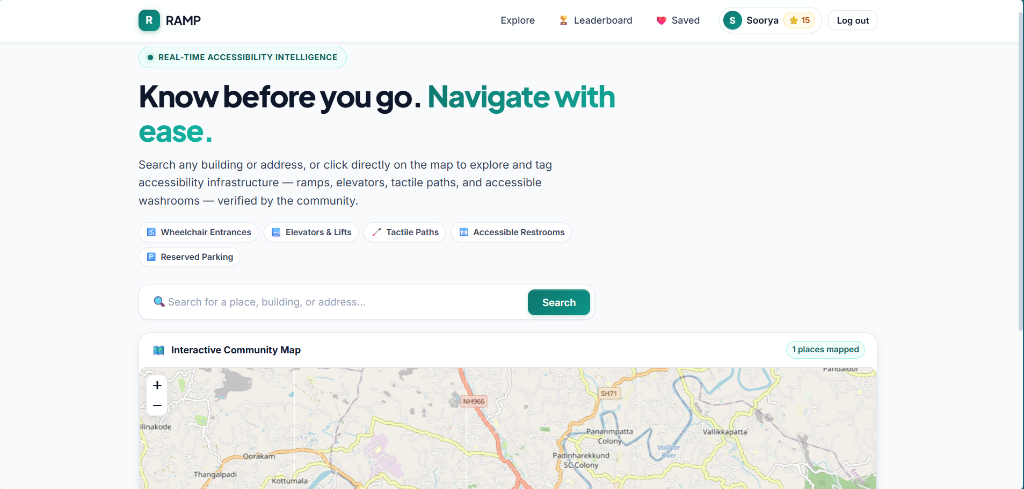
\includegraphics[width=0.92\textwidth]{home_landing.png}
\caption{RAMP Landing Page featuring Real-Time Community Map, Quick Trait Badges, and Geocoding Search}
\label{fig:screenshot_home}
\end{figure}

\noindent \textbf{Description}: 
Figure~\ref{fig:screenshot_home} illustrates the primary landing interface of RAMP. The presentation highlights real-time accessibility intelligence tags, quick-filter trait badges (Wheelchair Entrances, Elevators \& Lifts, Tactile Paths, Accessible Restrooms, and Reserved Parking), a location geocoding search input, and an interactive Leaflet GIS community map canvas with real-time mapped venue counters.

The interactive map is initialized with OpenStreetMap tile layers centered on regional urban coordinates. Users can search for venues or click directly on any coordinate to drop a pin and begin tagging accessibility infrastructure. The responsive search container connects to backend geocoding endpoints, converting text queries into geographic coordinates with fly-to camera animations. All interface elements feature high-contrast color tokens and ARIA labels compliant with WCAG~2.1~AA specifications.

% --- C.2 LOGIN / AUTHENTICATION ---
\clearpage
\subsection*{C.2 Contributor Authentication Interface}
\begin{figure}[htbp]
\centering
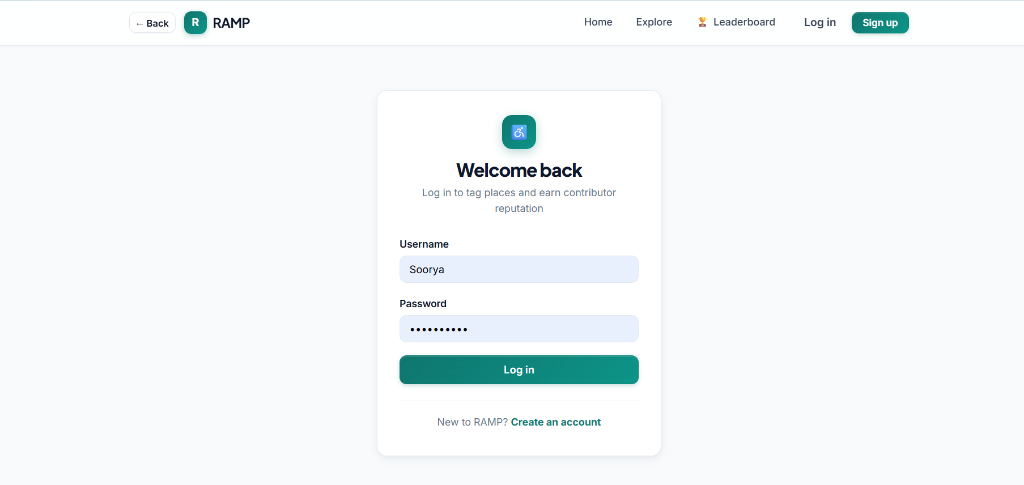
\includegraphics[width=0.68\textwidth]{login_screen.png}
\caption{User Authentication and Contributor Sign-in Screen}
\label{fig:screenshot_login}
\end{figure}

\noindent \textbf{Description}: 
Figure~\ref{fig:screenshot_login} showcases the contributor authentication interface featuring accessible form fields, password validation, and streamlined sign-in workflows. The authentication card is elevated using modern shadow tokens, featuring the brand emblem, accessible input labels, and clear error alert callouts.

Authentication is powered by JSON Web Tokens (SimpleJWT). Upon successful validation of credentials, the server issues a cryptographically signed access token and an HTTP-only refresh token. The client automatically stores these tokens and attaches bearer authorization headers to subsequent API calls via Axios interceptors. Authenticated contributors can map new venues, audit and verify peer-submitted measurements, accumulate reputation points, and customize personal accessibility profiles.

% --- C.3 EXPLORE PLACES DIRECTORY ---
\clearpage
\subsection*{C.3 Explore Accessible Places Directory}
\begin{figure}[htbp]
\centering
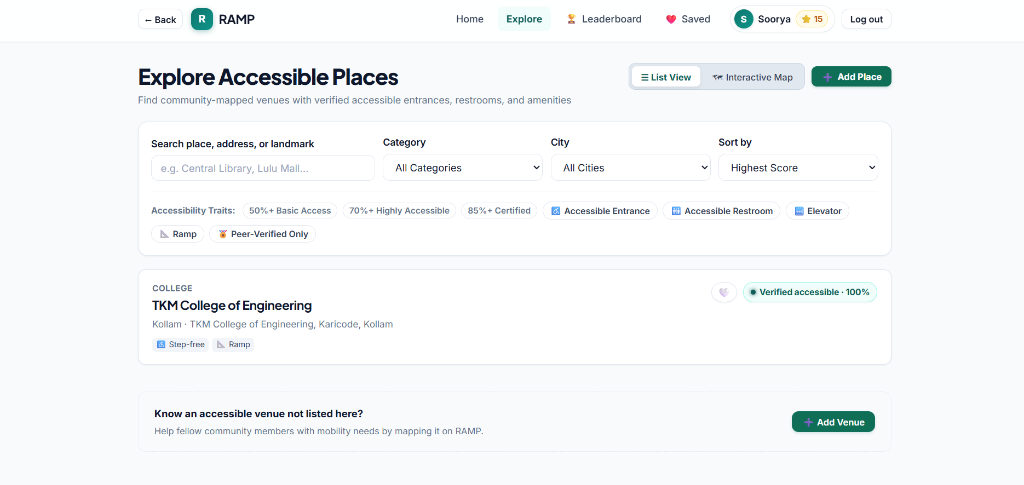
\includegraphics[width=0.92\textwidth]{explore_places.png}
\caption{Explore Venues Directory with Multi-Trait Accessibility Filtering and Verification Badges}
\label{fig:screenshot_explore}
\end{figure}

\noindent \textbf{Description}: 
Figure~\ref{fig:screenshot_explore} shows the primary exploration directory (\texttt{PlacesList.jsx}). The view integrates comprehensive filter criteria, including keyword search, category selector, city filter, score sorting, and physical trait chips (such as 50\%+ Basic Access, 70\%+ Highly Accessible, 85\%+ Certified, Accessible Restroom, Elevator, Ramp, and Peer-Verified Only).

Venue summary cards—such as the verified TKM College of Engineering entry—display calculated accessibility confidence percentages (100\% Verified Accessible), physical locations, amenity tags, and instant bookmarking controls. The interface provides a segmented control switcher allowing users to toggle seamlessly between a multi-card List View and a full-screen Interactive Map View. Filter operations execute as reactive parameters against the \texttt{/api/places/} endpoint with debounced queries.

% --- C.4 PLACE DETAIL & ENTRANCE AUDIT ---
\clearpage
\subsection*{C.4 Detailed Place Profile and Physical Entrance Audit}
\begin{figure}[htbp]
\centering
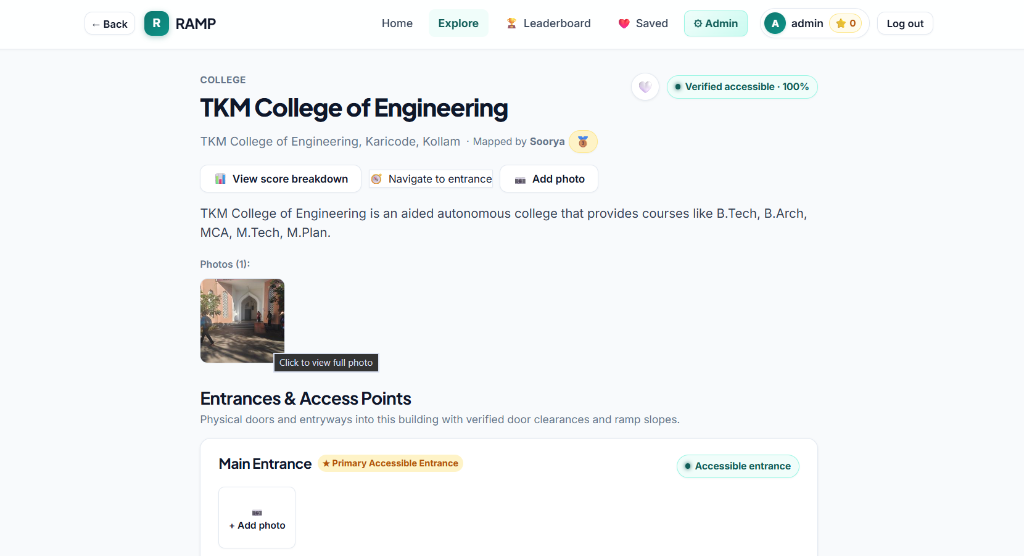
\includegraphics[width=0.92\textwidth]{place_detail.png}
\caption{Detailed Place Profile Displaying Verified Entrance Measurements and Photo Evidence}
\label{fig:screenshot_detail}
\end{figure}

\noindent \textbf{Description}: 
Figure~\ref{fig:screenshot_detail} illustrates the comprehensive venue detail dashboard (\texttt{PlaceDetail.jsx}) for an audited institution (TKM College of Engineering). The top header presents the venue category, official address, contributor attribution (Mapped by Soorya), and the composite accessibility confidence badge (100\% Verified Accessible). Primary action buttons allow visitors to view the Three-Pillar score breakdown, launch turn-by-turn navigation directly to the primary accessible entrance, or contribute photo evidence.

Below the header, the page presents verified entrance points with clear badges indicating the Primary Accessible Entrance. Each entrance card displays physical attributes, door clearances, ramp gradients, and photo evidence thumbnails. Visitors can click on any photo to launch the accessible full-screen image lightbox. Authenticated contributors are provided with interactive buttons to confirm or dispute individual physical traits, driving the crowdsourced peer-verification engine.

% --- C.5 MULTI-STEP VENUE ONBOARDING WIZARD ---
\clearpage
\subsection*{C.5 Multi-Step Venue Onboarding Wizard}
\begin{figure}[htbp]
\centering
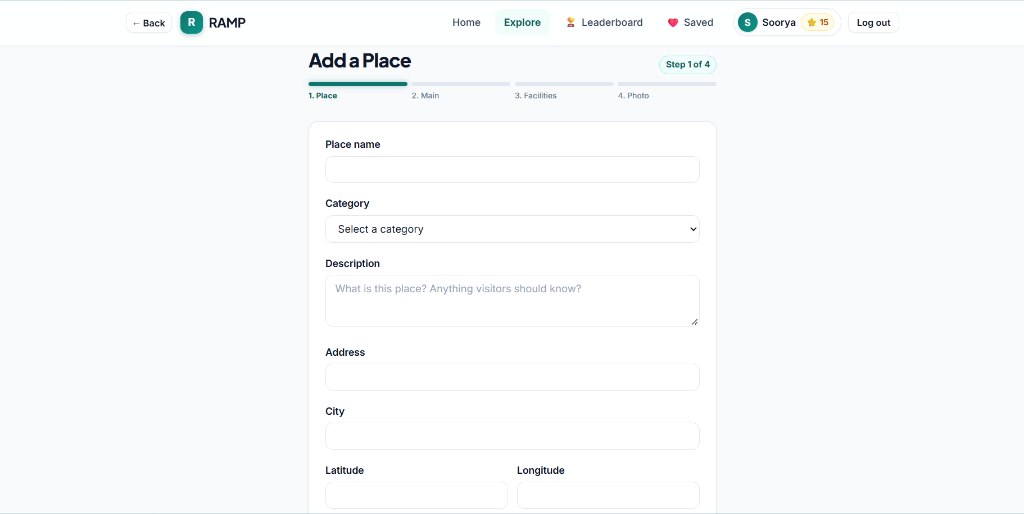
\includegraphics[width=0.72\textwidth]{add_place_wizard.png}
\caption{Multi-Step Venue Onboarding Wizard (Step 1: Place Details and Coordinates)}
\label{fig:screenshot_add_place}
\end{figure}

\noindent \textbf{Description}: 
Figure~\ref{fig:screenshot_add_place} displays the structured four-step venue contribution wizard (\texttt{AddPlace.jsx}). The visual progress bar tracks completion across Step~1 (Place Details and Geographic Coordinates), Step~2 (Main Entrance Parameters and Slope Gradients), Step~3 (Secondary Facilities and Amenities), and Step~4 (Evidence Photography).

When geographic coordinates are supplied (either typed or pinned directly from the Leaflet map), the system automatically initiates a background 50-meter spatial proximity check using PostGIS. If matching buildings are detected nearby, the user is presented with a warning card suggesting they add secondary facilities to the existing venue rather than creating duplicate entries. The step navigation ensures volunteer contributors provide accurate, high-integrity spatial data without cognitive overload.

% --- C.6 COMMUNITY LEADERBOARD & ACHIEVEMENTS ---
\clearpage
\subsection*{C.6 Community Leaderboard and Contributor Recognition}
\begin{figure}[htbp]
\centering
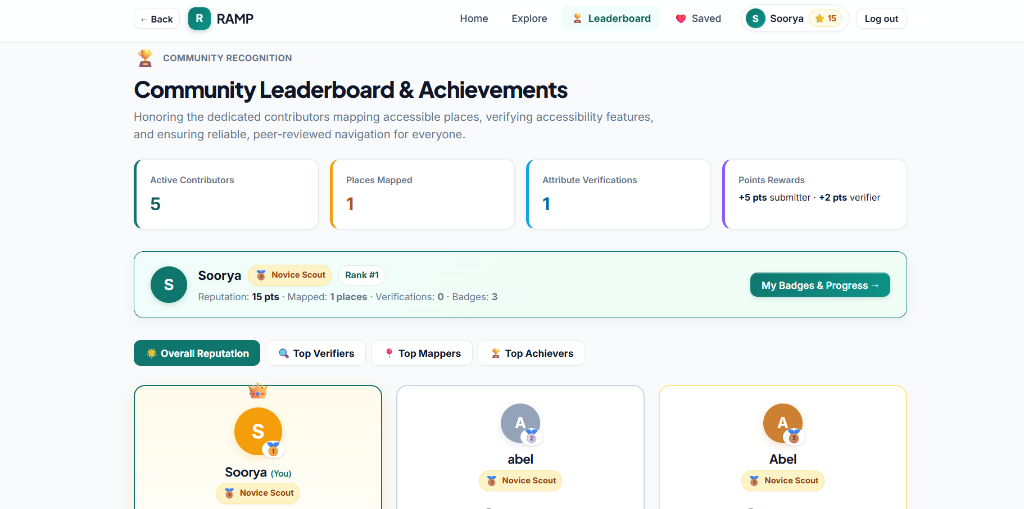
\includegraphics[width=0.92\textwidth]{leaderboard_gamification.png}
\caption{Community Leaderboard, Contribution Metrics, and Contributor Recognition Podium}
\label{fig:screenshot_leaderboard}
\end{figure}

\noindent \textbf{Description}: 
Figure~\ref{fig:screenshot_leaderboard} illustrates the gamified community engagement dashboard (\texttt{Leaderboard.jsx}). Global metric tiles display active contributors, total places mapped, attribute verifications, and point rewards (+5 points for submissions, +2 points for audits).

The user's personalized banner highlights their active tier (Novice Scout), rank position (Rank \#1 Soorya), reputation points, and unlocked badges, accompanied by a dynamic podium recognizing top contributors across overall reputation, peer verification, and mapping milestones. The gamification mechanics motivate volunteers to conduct meticulous physical audits and participate in peer-verification workflows, preventing contributor drop-off over extended project lifecycles.

% --- C.7 ADMINISTRATIVE MODERATION PORTAL ---
\clearpage
\subsection*{C.7 Ten-Panel Administrative Moderation Portal}
\begin{figure}[htbp]
\centering
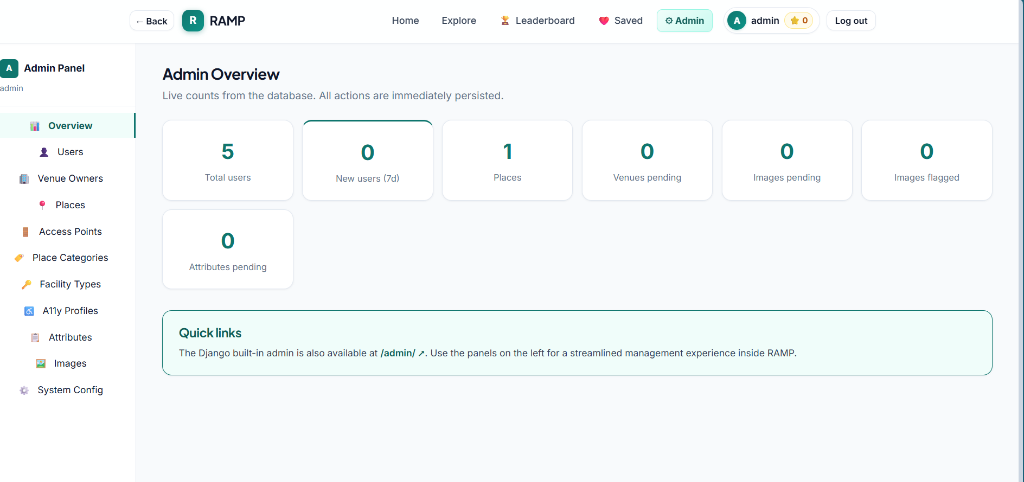
\includegraphics[width=0.92\textwidth]{admin_overview.png}
\caption{Administrative Moderation Portal Overview Displaying Operational Metrics and Navigation Panels}
\label{fig:screenshot_admin}
\end{figure}

\noindent \textbf{Description}: 
Figure~\ref{fig:screenshot_admin} showcases the centralized 10-panel Administrative Moderation Portal (\texttt{Admin.jsx}) accessible exclusively to staff and system administrators. The overview dashboard summarizes real-time operational database counts: Total Users, Places Mapped, Venues Pending Moderation, Images Flagged, and Attributes Pending Verification.

The left sidebar navigation provides instant access to 10 specialized administrative modules: Users, Venue Owners, Places, Access Points, Place Categories, Facility Types, Accessibility Profiles, Attributes, Images, and System Config. Through these panels, administrators can moderate flagged photographs, inspect disputed physical measurements, update operational parameters dynamically, and maintain complete governance over crowdsourced data.

\end{document}
